% $Id: introduction.tex 65669 2015-01-09 14:55:20Z tgershon $

\section{Theory}
\label{sec:Theory}

%Why loops no FCNC
%why suppressed
%Decay Rate formalism
%Make point of sum of diagrams

As mentioned previously \lhcb predominantly searches for new physics (NP) indirectly through measurements of observable quantities.  One of these quanitites is decay rates, which is the subject of the analysis presented in section \ref{sec:Analysis} of this report.  In general, the differential decay rate of a specific particle decay is given by,
\begin{equation}
  \label{eq:fgr}
  d\Gamma(P_A\to1 + ......n) = \frac{|\mathscr{M}|^2}{2M_A}dQ
\end{equation}

where $M_A$ is the mass of the decaying particle, $dQ$ is the lorentz invariant phase space (LIPS) and $|\mathscr{M}|^2$ is the matrix element for that decay \cite{halzen1984quarks}.  The phase space factor arises from the fact the decay rate is a function of the final state particles momenta, and there is a continuous range of momenta the final state particles can take.  One can calculate the LIPS and insert it into equation \ref{eq:fgr}, giving a differential decay rate for a general $n$ body decay to be,
\begin{equation}
  \label{eq:diffdec}
  d\Gamma(P_A \to 1+ .....n) = \frac{1}{2M_A}\bigg(\prod_{f}^{N}\frac{\vec{d^3p}_f}{(2\pi)^3(2E_f)}\bigg)|\mathscr{M}|^2(2\pi)^4\delta^4\bigg(\sum_{f}^n(p_f)-p_A\bigg)
\end{equation}
where the subscript f represents a final state particle and A is the initial particle \cite{halzen1984quarks}. The product over all final state particles in equation \ref{eq:diffdec} takes into account the available phase space and the dirac delta function ensures four momenta conservation.  One can then integrate over all possible momenta $p_1...p_n$ to get a total decay rate.

The interesting part of equation {\ref{eq:diffdec}} is the matrix element, $|\mathscr{M}|$.  This governs the fundamental interaction and transforms the initial state particles to the final state of the system.  For the decay of a particle $P_A$ to a given final state there is almost always more than one way in which the decay can proceed meaning more than one Feynman diagram can be drawn for the given decay.  Each Feynman diagram has an associated decay amplitude that is the reuslt of a perturbative calculation.  However, this can be simplified with the use of Feynman rules which assign vertex factors and propagator terms to the pictorial representation.  The total matrix element $\mathscr{M}$ is then given by,

\begin{equation}
  \label{eq:matrix}
  |\mathscr{M}|^2=|\sum_i A_i|^2
\end{equation}

where $A_i$ is the amplitude calculated from an individual Feynman diagram.  The consequences of this are that every possible feynman diagram contributes to the observable decay rate, although some provide negligable contributions.

As flavour changing neutral currents are forbidden in the standard model, the b \to s quark flavour transistions must take place via an electroweak loop.  An example of a decay involving such a b to s transistion is shown in figure \ref{fig:btos}.

\begin{figure}
  \centering
  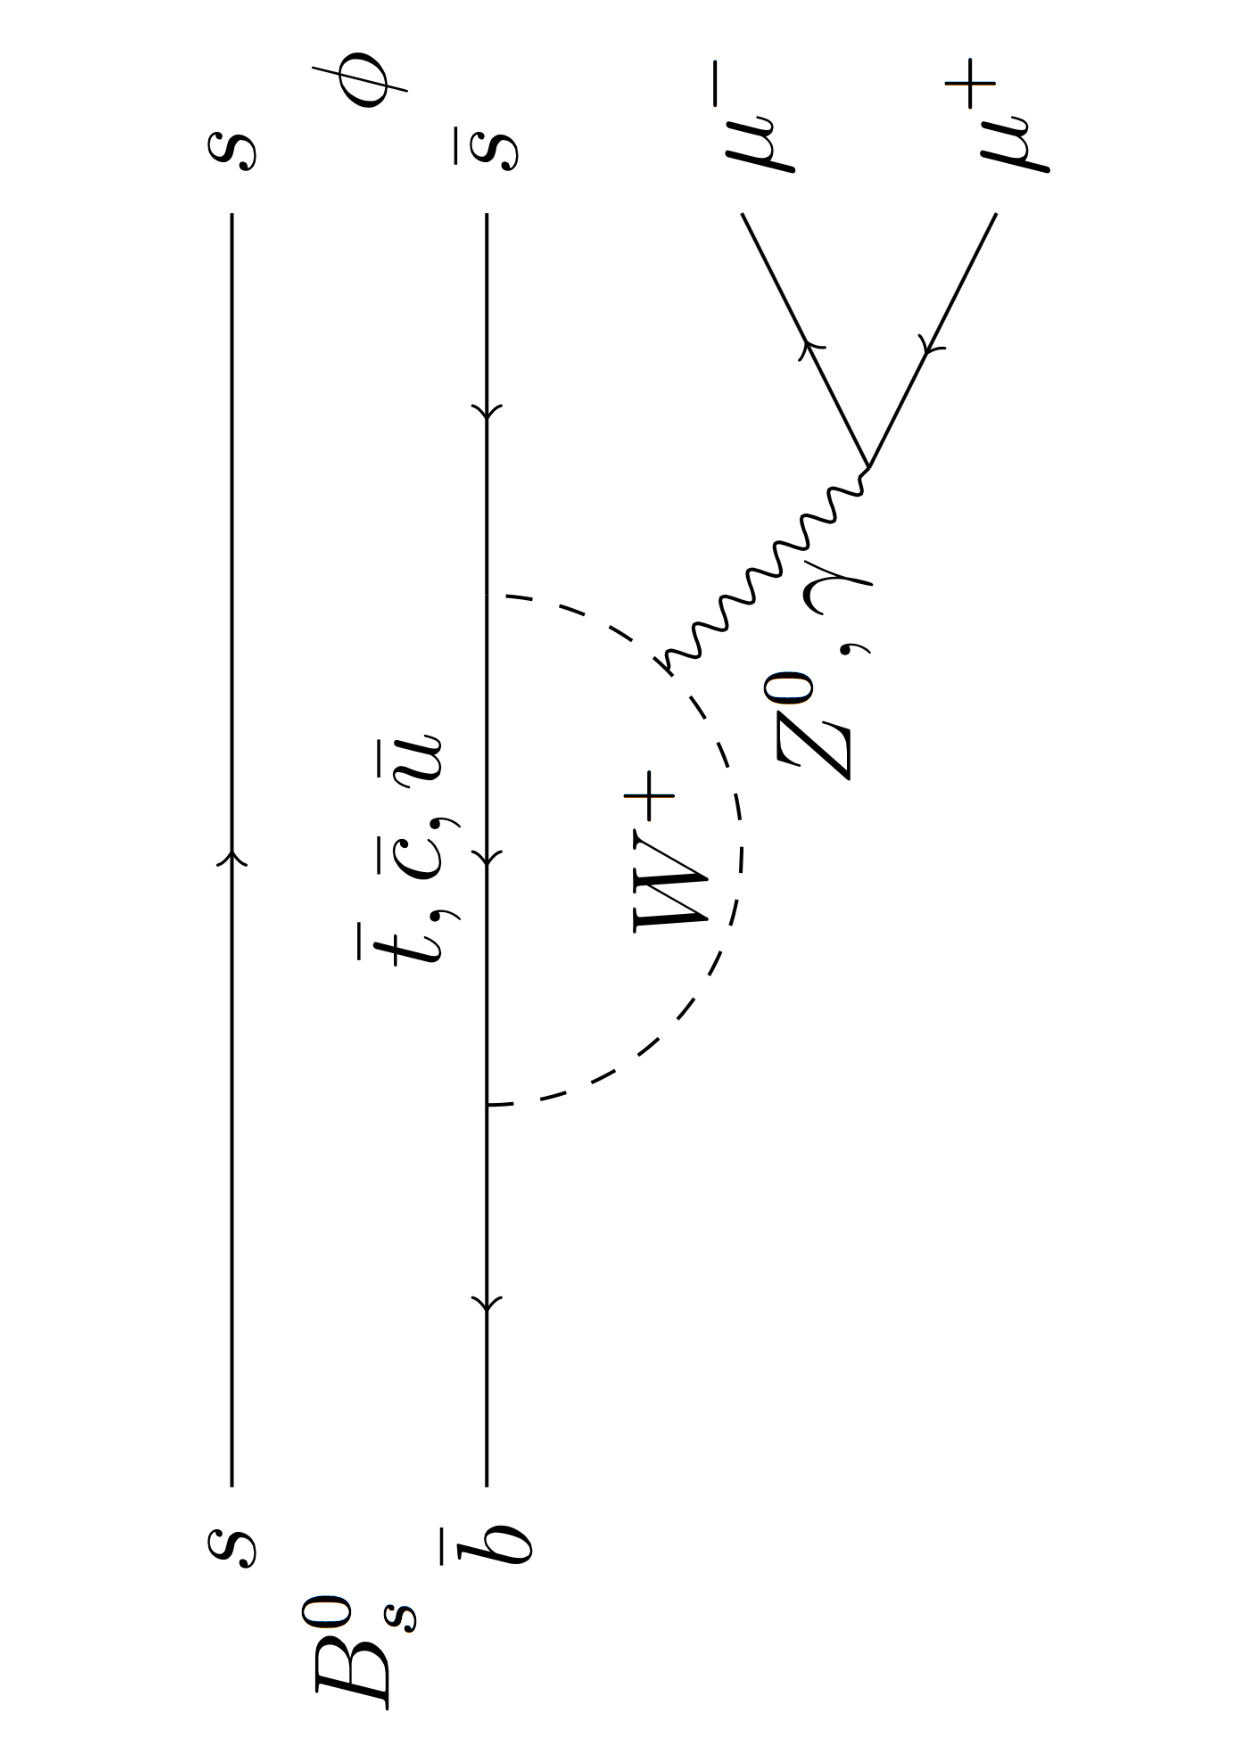
\includegraphics[width=0.5\textwidth,angle=270]{Bsphimumu.pdf}
  \caption{A feynman diagram for the decay of \Bs \to $\phi \mu \mu$ via an electroweak loop \cite{LHCb-PAPER-2013-017}.}
  \label{fig:btos}
\end{figure}

Here, a virtual W+ boson is created from the vacuum which changes the flavour of the b quark to any of the up type quarks which then recombines with the W+ boson to create an s quark, giving an overall change from a b flavour quark to an s flavoured quark.  Although theoretically it can be any of the up type quarks that meidates the loop, the top quark provides the dominant contribution due to its large mass.

As the total decay rate is the sum of all amplitudes, as shown in equation \ref{eq:matrix}, the overall matrix element for an electroweak loop has to include all possible mediators of the loop.  If NP beyond the standard model exists, it could enter as a mediator of loop diagrams.  In this case, the W+ boson could be replaced with a beyond the standard model heavy vector boson or the loop could be replaced with pair produced super symmetric particles.  In any case of NP entering into the loop, it would add another amplitude to the matrix element calculation.  Consequently, the total decay rate would be different and the standard model prediction would no longer be correct.  Therefore, by measuring decay rates (or in practice branching fractions) and comparing results to standard model predictions an indirect search for new physics can be performed.

One of the main advantages of indirect searches is that they offer sensitivity to NP at energies higher than what is accessible through direct searches.  Also, they are sensitive to a wider range of NP effects rather than just the target of the search being performed.  However, loop decays are heavily suppressed in the standard model due to the extra vertex factors they introduce to the decay amplitude.  This makes loop decays rare, meaning large data samples and high detection efficiencies are needed to study them with any precision.








